\chapter{Appendix} \label{chapter: Appendix}

\begin{code}[htpb]
    \centering
    \begin{tabular}{c}
    \begin{lstlisting}[language=ruby]
apiVersion: apps/v1
kind: DaemonSet
metadata:
    name: green-daemon
    namespace: default
spec:
    selector:
        matchLabels:
            name: green-daemon
    template:
        metadata:
            labels:
                name: green-daemon
        spec:
            containers:
            - name: green
              image: led-daemon
              args:
              - GREEN
            nodeSelector:
                type: "virtual-kubelet"
                model: "raspberry-pi"
                light: "GREEN"
            tolerations:
            - key: "virtual-kubelet.io/provider"
              operator: "Equal"
              value: "unikernel"
              effect: "NoSchedule"
  \end{lstlisting}
  \end{tabular}
  \caption{Green-daemon specification}\label{fig:green-daemon}
  \end{code}


\begin{code}[htpb]
    \centering
    \begin{tabular}{c}
    \begin{lstlisting}[language=ruby]
apiVersion: apps/v1
kind: Deployment
metadata:
    name: humidity
    labels:
        app: humidity
spec:
    selector:
        matchLabels:
            app: humidity
    template:
        metadata:
            labels:
                app: humidity
        spec:
            containers:
            - name: unikernel
              image : sensor.native
              env:
              - name: "sensor"
                value: "humidity"
            nodeSelector:
                type: "virtual-kubelet"
                model: "raspberry-pi"
            tolerations:
            - key: "virtual-kubelet.io/provider"
              operator: "Equal"
              value: "unikernel"
              effect: "NoSchedule"
\end{lstlisting}
\end{tabular}
\caption{Unikernel specific deployment}\label{fig:unikernel-dep}
\end{code}

\iffalse
  \begin{figure}
    \centering
    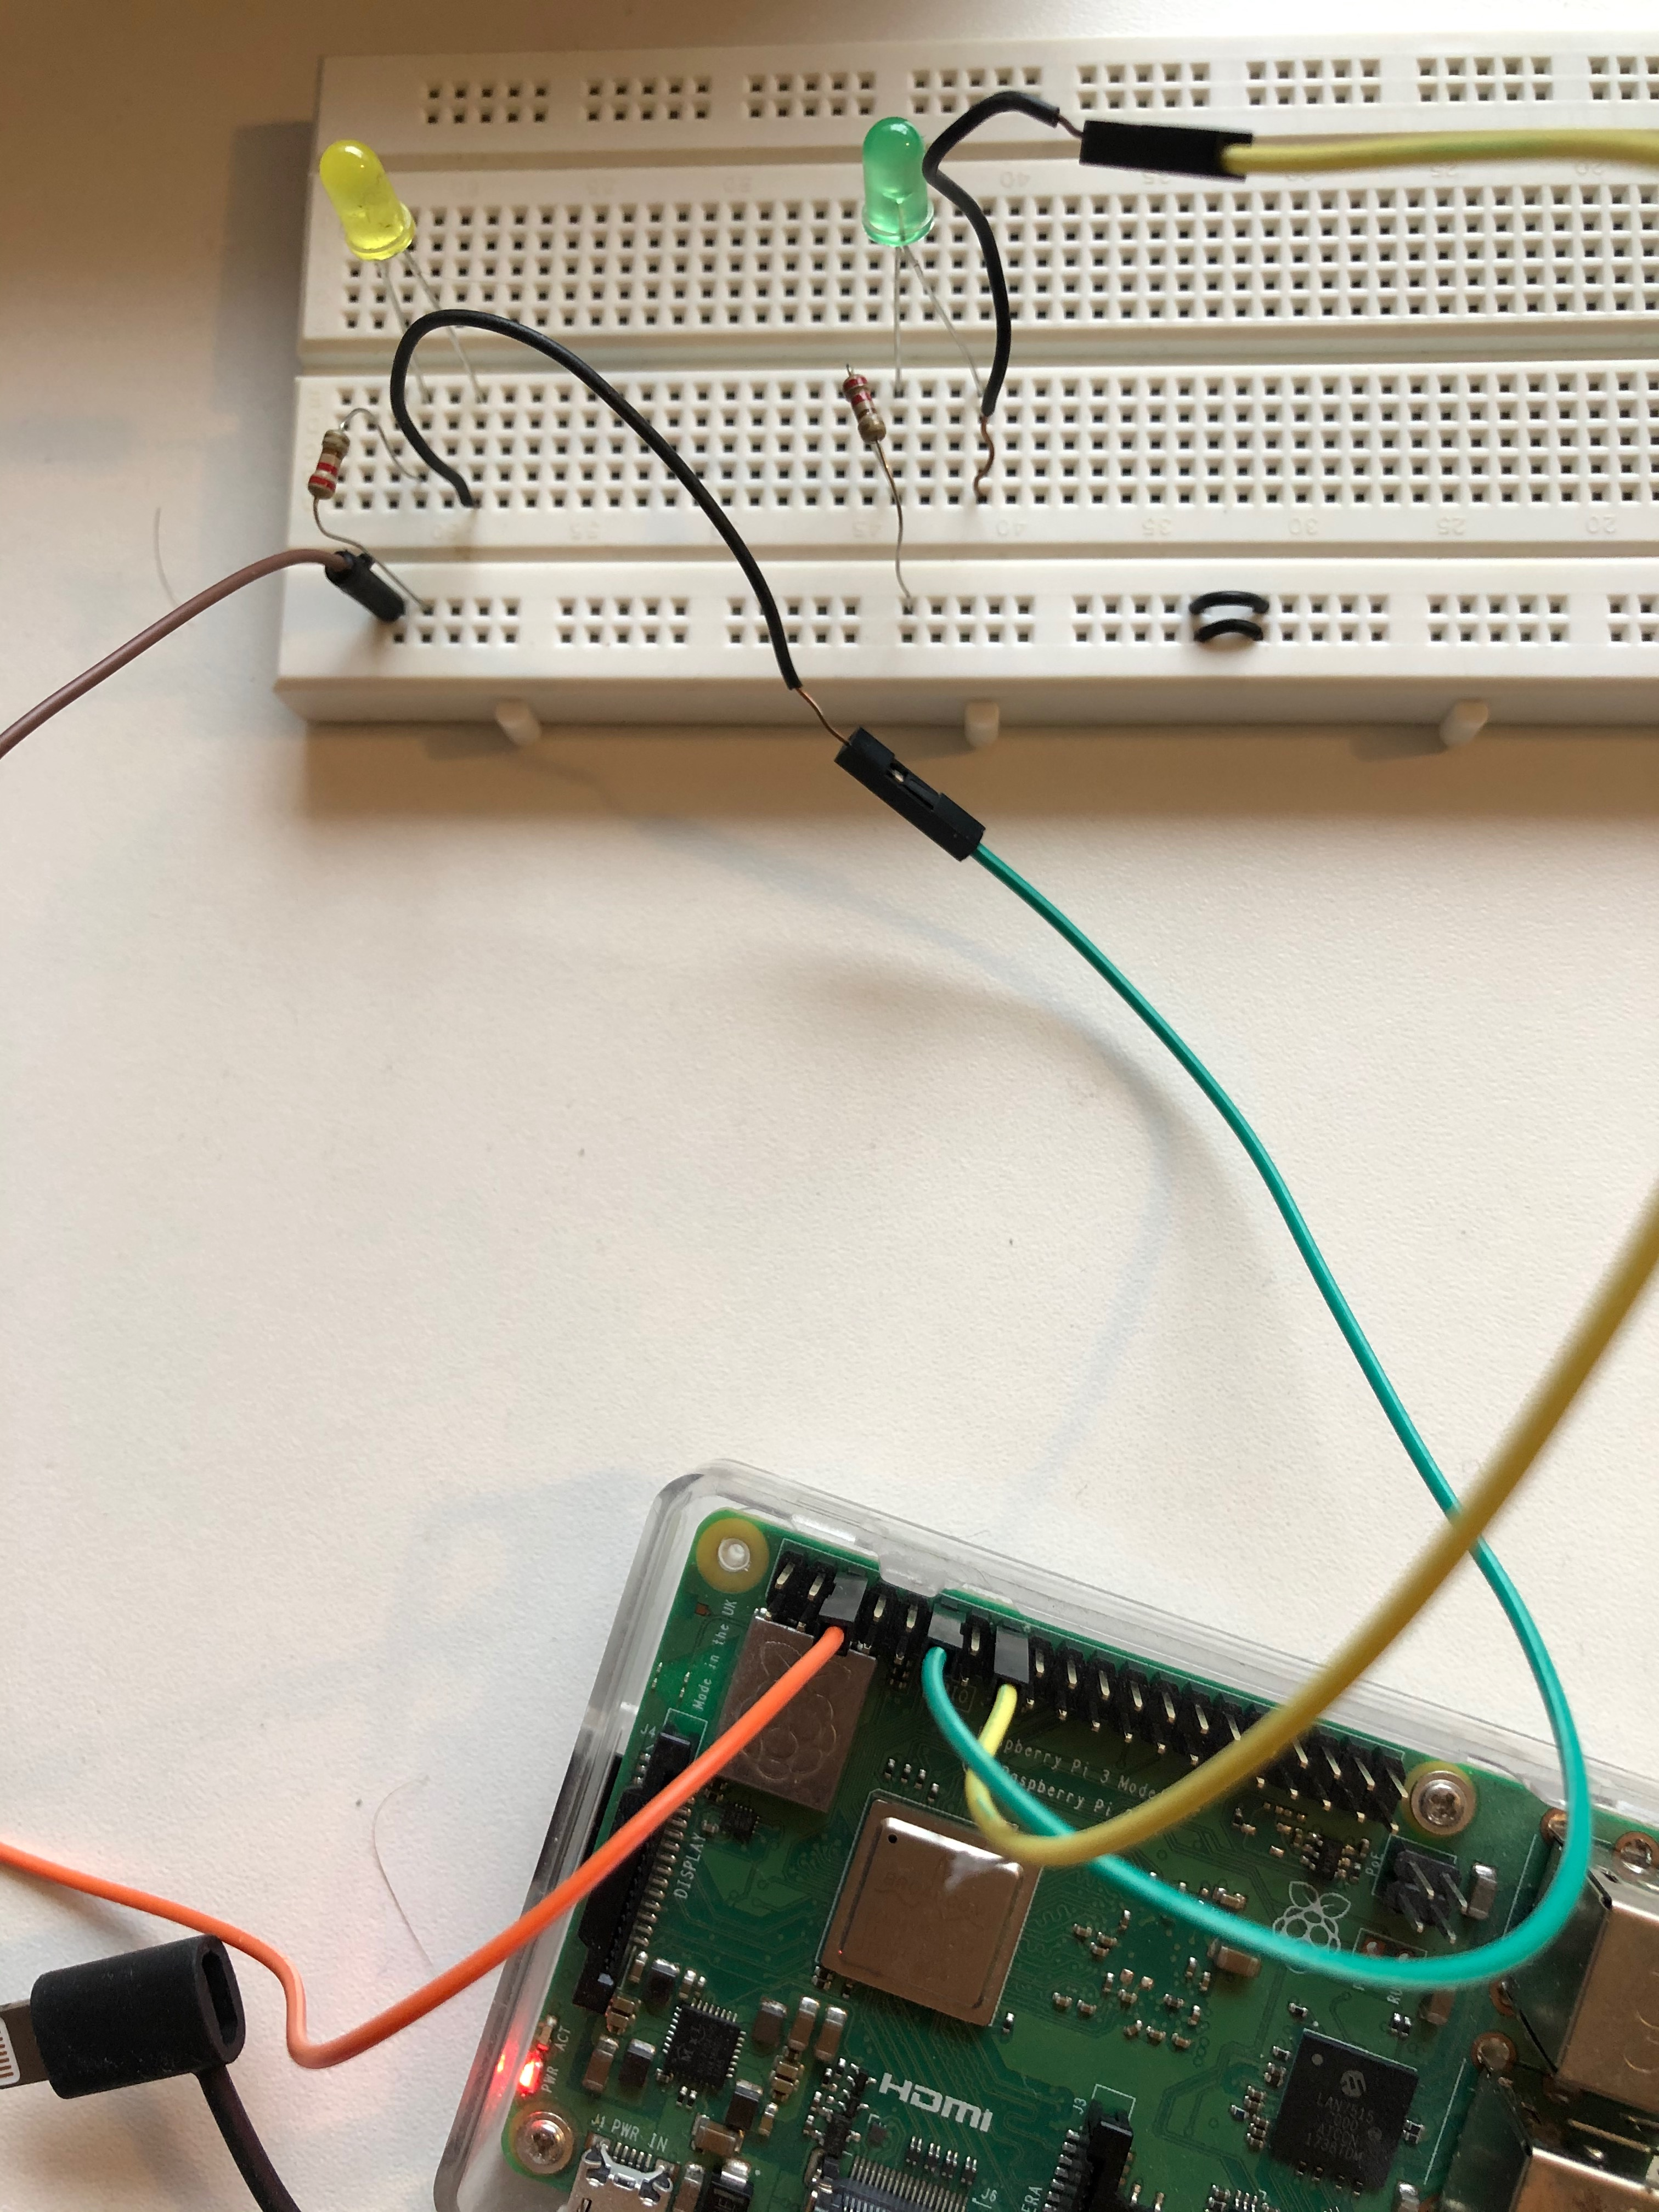
\includegraphics[width=0.9\textwidth]{rasp-running.jpeg}
    \caption{Photo of wiring of \ref{fig:rpi-diagram}}\label{fig:wiring}
  \end{figure}
\fi